\documentclass[runningheads]{llncs}

\usepackage[T1]{fontenc}
\usepackage{lmodern}
\usepackage{graphicx}
\usepackage{amsmath}
\usepackage{amssymb}
\usepackage{booktabs}
\usepackage{array}
\usepackage{tabularx}
\usepackage{url}
\usepackage{color}
\usepackage{hyperref}
\hypersetup{hidelinks}
\usepackage{microtype}
\usepackage{tikz}
\usetikzlibrary{shapes.geometric, arrows, positioning}
\renewcommand\UrlFont{\color{blue}\rmfamily}
\setlength{\emergencystretch}{1em}

\title{Explainable Quantum-Inspired Multi-label Classification of Non-Functional Requirements}
\titlerunning{Explainable Quantum-Inspired Multi-label NFR Classification}

\author{Nguyen Hoang Phuc\inst{1}\thanks{Corresponding author.} \and
Nguyen Le Quynh Giang\inst{1} \and
Le Doan Gia Hung\inst{1} \and
Lai Duc Hung\inst{1}}
\authorrunning{N. H. Phuc et al.}

\institute{FPT University, Ho Chi Minh City, Vietnam \\
\email{nphuc4748@gmail.com, nguyengiang14012005@gmail.com,\\
lhung291005@gmail.com, hungld@fpt.edu.vn}}

\begin{document}
\maketitle

\begin{abstract}
Non-functional requirements (NFRs) frequently overlap across quality attributes
such as security, performance, usability, and availability, making NFR
classification a natural multi-label problem. This paper presents an
intrinsically explainable quantum-inspired method for multi-label NFR
classification. Requirements are represented as normalized semantic states,
NFR labels as projection directions, and label scores as squared projection
amplitudes; a label interference matrix models NFR co-occurrence, and
token-level amplitude contributions explain predictions without a post-hoc
explainer. The paper also gives a theoretical characterization of the deployed
decision rule, identifying when the quantum-inspired geometry reduces to
cosine-style ranking and when interference, or positive-model row-wise
normalization, creates genuine cross-label coupling. We evaluate
quantum-inspired variants on the
NICE multi-label dataset against TF-IDF Logistic Regression, TF-IDF Linear SVM,
Sentence-BERT, fine-tuned DistilBERT, and a label-frequency baseline. Under
5-fold cross-validation, Sentence-BERT achieves the highest Macro-F1; the
hybrid quantum--SVM model is competitive with TF-IDF baselines and obtains the
highest Macro-F1 among non-embedding models, but its advantage is not
statistically significant at this dataset size. The main contribution is
therefore not a state-of-the-art accuracy claim, but an interpretable
multi-label scoring formulation, a precise account of when its geometry helps
or collapses to classical behavior, and a deletion-based faithfulness
evaluation of its intrinsic token explanations.
\keywords{Requirements Engineering \and Non-Functional Requirements \and Multi-label Classification \and Quantum-inspired Model \and Explainable AI \and Software Engineering}
\end{abstract}

\section{Introduction}
Requirements Engineering (RE) is a critical activity in software development
because requirement quality strongly affects downstream architecture,
implementation, testing, and maintenance decisions. Among requirement types,
non-functional requirements (NFRs) are particularly difficult to identify and
classify automatically. NFRs describe quality attributes such as security,
performance, usability, availability, scalability, and maintainability. Unlike
many functional requirements, NFRs are often ambiguous, context-dependent, and
overlapping.

For example, a requirement stating that payment information must be encrypted
and accessible only to authorized administrators clearly relates to security. If
the same requirement also constrains availability, auditability, or response
time, it may express multiple NFR categories at once. Therefore, NFR
classification is better treated as a multi-label problem rather than a strict
single-label problem \cite{tsoumakas2007multilabel,zhang2014review}.

This paper investigates the research topic: \emph{Explainable Quantum-Inspired
Multi-label Classification of Non-Functional Requirements}. The key idea is to
represent each requirement as a semantic state and estimate its degree of
association with multiple NFR labels using projection amplitudes. The approach
is quantum-inspired rather than quantum-hardware-based: it runs on ordinary
computers and borrows mathematical intuitions such as state representation,
projection amplitude, and interference from geometric information retrieval and
quantum language modeling \cite{vanrijsbergen2004geometry,sordoni2013quantum,li2019cnm}.

The paper's positive claim is that this formulation provides an intrinsic
explanation mechanism for multi-label NFR classification and a testable
theory of when quantum-inspired geometry changes the decision rule. The basic
projection component is closely related to centroid-based text classification;
the interference and positive-model row-wise normalization analyses make
explicit when the model becomes more than an independent centroid classifier
and when it does not. Empirically, the hybrid model offers a small, suggestive
accuracy gain over comparable TF-IDF baselines, while the primary value of the
method lies in its transparent scoring structure and diagnostic ablation.

The contributions of this paper are:
\begin{itemize}
    \item an intrinsically explainable quantum-inspired formulation for multi-label NFR classification;
    \item a theoretical characterization of interference and, for the positive-projection model, row-wise normalization as two sources of cross-label coupling;
    \item token-level semantic amplitude explanations evaluated with a deletion-based ERASER faithfulness test;
    \item empirical comparison against TF-IDF Logistic Regression, TF-IDF Linear SVM, Sentence-BERT, fine-tuned DistilBERT, and a label-frequency baseline on the NICE dataset;
    \item an ablation study showing where projection type, label interference, and hybrid fusion weight help or fail.
\end{itemize}

\section{Related Work}
Automated NFR classification includes early rule and supervised-learning work
on security, performance, usability, and related quality attributes
\cite{clelandhuang2007automated,kurtanovic2017automatically,dalpiaz2019requirements}.
PROMISE and PROMISE-expanded support repeatable NFR experiments
\cite{mitrevski_promise_exp}, while NICE provides the multi-label NFR setting
used here \cite{nice_dataset,nice_preprint}. Because label filtering, splits,
and metrics differ from the NICE paper, we report all baselines on the same
downloaded data.

Our baselines cover TF-IDF classifiers, which remain strong in small text
datasets \cite{sebastiani2002machine}, and transformer-based representations,
including BERT-style transfer learning, NoRBERT, and Sentence-BERT
\cite{devlin2019bert,hey2020norbert,reimers2019sentencebert}. The
quantum-inspired component follows geometric information retrieval and
quantum-inspired language modeling, where matching is expressed through vector
spaces, projections, and wave-function-inspired representations
\cite{vanrijsbergen2004geometry,sordoni2013quantum,zhang2018quantum,li2019cnm}.
For explainability, we relate to LIME, SHAP, and ERASER-style rationale
evaluation \cite{ribeiro2016lime,lundberg2017shap,deyoung2020eraser}.

\section{Research Questions}
This study is guided by three research questions:

\textbf{RQ1.} Can a quantum-inspired semantic projection model classify
multi-label NFRs competitively compared with classical and embedding baselines?

\textbf{RQ2.} Does the model provide useful explainability through token-level
semantic amplitude contributions?

\textbf{RQ3.} Is the observed behavior stable under cross-validation rather than
only in a single train/test split?

\section{Proposed Method}

Figure~\ref{fig:architecture} summarizes the complete prediction pipeline and
the point at which the quantum-inspired and classical branches are fused.

\begin{figure}[tbp]
\centering
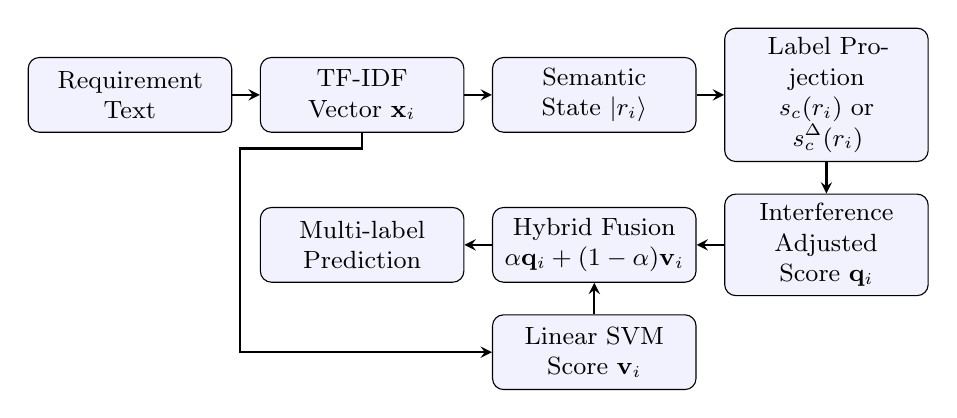
\begin{tikzpicture}[
  box/.style={draw, rectangle, rounded corners, minimum height=2.7em,
    text width=2.35cm, align=center, fill=blue!5, font=\small},
  arrow/.style={thick,->,>=stealth}
]
\node[box] (req) {Requirement Text};
\node[box, right=0.35cm of req] (tfidf) {TF-IDF Vector $\mathbf{x}_i$};
\node[box, right=0.35cm of tfidf] (state) {Semantic State $\lvert r_i \rangle$};
\node[box, right=0.35cm of state] (proj) {Label Projection\\$s_c(r_i)$ or\\$s^{\Delta}_c(r_i)$};
\node[box, below=0.4cm of proj] (interf) {Interference\\Adjusted Score $\mathbf{q}_i$};
\node[box, left=0.35cm of interf] (hybrid) {Hybrid Fusion\\$\alpha\mathbf{q}_i+(1-\alpha)\mathbf{v}_i$};
\node[box, left=0.35cm of hybrid] (pred) {Multi-label Prediction};
\node[box, below=0.4cm of hybrid] (svm) {Linear SVM\\Score $\mathbf{v}_i$};

\draw[arrow] (req) -- (tfidf);
\draw[arrow] (tfidf) -- (state);
\coordinate (svmroute) at ([xshift=-0.25cm]pred.west);
\draw[arrow] (tfidf.south) -- ++(0,-0.2) -| (svmroute) |- (svm.west);
\draw[arrow] (state) -- (proj);
\draw[arrow] (proj) -- (interf);
\draw[arrow] (interf) -- (hybrid);
\draw[arrow] (svm) -- (hybrid);
\draw[arrow] (hybrid) -- (pred);
\end{tikzpicture}
\caption{Hybrid quantum-inspired multi-label classification pipeline. A
requirement is transformed into a TF-IDF vector and normalized semantic state,
then projected onto NFR-label directions. Co-occurrence interference adjusts
the projection scores; the resulting quantum-inspired scores are fused with
Linear SVM scores and thresholded to produce the multi-label prediction.}
\label{fig:architecture}
\end{figure}

\subsection{Requirement Representation}
Each requirement text is first converted into a TF-IDF vector:
\begin{equation}
    \mathbf{x}_i \in \mathbb{R}^{d},
\end{equation}
where $d$ is the vocabulary size. The vector is normalized to form a semantic
state:
\begin{equation}
    \lvert r_i \rangle = \frac{\mathbf{x}_i}{\left\|\mathbf{x}_i\right\|_2}.
\end{equation}
This normalization allows the requirement to be interpreted as a direction in
semantic space.

\subsection{Label Projection}
For each NFR label $c$, a label basis vector is estimated from the centroid of
positive training examples:
\begin{equation}
    \lvert c \rangle = \frac{1}{N_c}\sum_{i:y_{ic}=1}\lvert r_i \rangle,
\end{equation}
followed by normalization. The raw association between requirement $r_i$ and
label $c$ is computed as a squared projection amplitude:
\begin{equation}
    s_c(r_i) = \left(\langle c \mid r_i \rangle\right)^2.
\end{equation}
We call $s_c(r_i)$ an association score rather than a probability because the
scores over labels are not constrained to sum to one.

\subsection{Contrastive Label Projection}
The positive-only centroid projection is simple and interpretable, but it does
not explicitly model how a label differs from other labels. Therefore, this
work also evaluates a contrastive quantum-inspired variant. For each label $c$,
the contrastive direction is computed as:
\begin{equation}
    \lvert c_{\Delta} \rangle =
    \frac{\mu_c^{+} - \mu_c^{-}}
    {\left\|\mu_c^{+} - \mu_c^{-}\right\|_2},
\end{equation}
where $\mu_c^{+}$ is the centroid of requirements that contain label $c$, and
$\mu_c^{-}$ is the centroid of requirements that do not contain label $c$.
Unlike the positive centroid vector, the contrastive direction is signed: a
requirement can project in the opposite direction of a label. Squaring a
negative projection would incorrectly assign a high score to evidence against
the label. Therefore, the contrastive variant uses a half-wave rectified
projection score:
\begin{equation}
    s^{\Delta}_c(r_i) =
    \left(\max(0,\langle c_{\Delta}\mid r_i\rangle)\right)^2.
\end{equation}
This preserves positive alignment with the label direction while suppressing
opposite-direction evidence.

\subsection{Interference Adjustment}
To reflect label co-occurrence, the model estimates a label interference matrix
from training labels. Let $N_{kl}$ be the number of training samples containing
both labels $k$ and $l$, and let $N_k$ be the number of samples containing label
$k$. The normalized co-occurrence matrix is:
\begin{equation}
    M_{kl} = \frac{N_{kl}}{N_k},
\end{equation}
with the diagonal set to 1. The implementation mixes this matrix with the
identity matrix:
\begin{equation}
    \mathbf{M}' = (1-\lambda)\mathbf{I} + \lambda\mathbf{M},
\end{equation}
where $\lambda$ controls interference strength. For projection scores
$\mathbf{p}_i$, adjusted scores are computed as:
\begin{equation}
    \mathbf{s}_i = \mathrm{normalize}(\mathbf{p}_i \mathbf{M}').
\end{equation}
For the positive-projection model, $\mathrm{normalize}(\cdot)$ denotes row-wise
min--max normalization into $[0,1]$. For the contrastive model, the rectified
projection is passed through a sigmoid calibration and the interference-adjusted
scores are clipped into $[0,1]$. The resulting scores are association scores
for thresholding rather than mutually exclusive probabilities.

\subsection{Hybrid Quantum--SVM Fusion}
To improve stability on small and imbalanced datasets, a hybrid model combines
the contrastive quantum-inspired score with a one-vs-rest Linear SVM score:
\begin{equation}
    \mathbf{h}_i = \alpha \mathbf{q}_i + (1-\alpha)\mathbf{v}_i,
\end{equation}
where $\mathbf{q}_i$ is the contrastive quantum-inspired score vector,
$\mathbf{v}_i$ is the calibrated SVM score vector, and $\alpha$ is the quantum
fusion weight. In the final experiments, $\alpha=0.30$ is used as a moderate
quantum weight; the ablation study (Table~\ref{tab:nice-ablation}) shows that
Macro-F1 is not sensitive to the exact value in this range ($\alpha=0.15$,
$0.30$, and $0.50$ are within one standard deviation of each other), so
$\alpha=0.30$ was kept as a round, non-edge value rather than as a value
selected for maximizing cross-validation Macro-F1.

\subsection{Explainability}
For a predicted label $c$, token-level contribution is estimated from the
element-wise product between the requirement state and the label basis:
\begin{equation}
    e_{ijc} = r_{ij}c_j.
\end{equation}
Terms with the largest absolute contributions are reported as explanations. In
the experiments, these explanations are generated by the rectified contrastive
projection model. We evaluate them using a deletion test: if the highlighted
terms are faithful, deleting them should reduce the model score more than
deleting random nonzero terms.

\subsection{Theoretical Characterization}
The purpose of this analysis is boundary characterization rather than a claim
that every quantum-inspired mechanism improves the recommended hybrid model.
It identifies which operations create behavior beyond independent centroid
scoring and which collapse to classical geometry. The positive-projection
formulation exposes two mechanistically distinct
sources of cross-label coupling in its deployed decision rule: the interference
matrix (Proposition~\ref{prop:interference}) and the row-wise score
normalization applied by this variant before thresholding
(Proposition~\ref{prop:reduction}). Only the within-instance \emph{ranking}
of labels reduces to a cosine-similarity ranking; the thresholded binary
decision of this variant does not reduce to $L$ independent per-label centroid
classifiers, even when interference is switched off. The contrastive and hybrid
variants instead use sigmoid-calibrated scores without row-wise min--max
normalization, so Proposition~\ref{prop:reduction} does not apply to them. For
the recommended hybrid, Proposition~\ref{prop:interference} characterizes its
quantum branch, but the ablation later shows that this coupling is weak or
harmful on NICE; its theoretical value is therefore to delimit a mechanism,
not to present that mechanism as the source of the hybrid's empirical result.

\begin{proposition}[Interference as label coupling]
\label{prop:interference}
With $\mathbf{M}'=(1-\lambda)\mathbf{I}+\lambda\mathbf{M}$, the pre-normalization
score for label $l$ has the form
\begin{equation}
    u_l \propto (1-\lambda)p_l + \lambda\sum_k p_k M_{kl}.
\end{equation}
The second term injects score mass from co-occurring labels $k$, where
$M_{kl}=N_{kl}/N_k$. This coupling cannot be represented by a diagonal
per-label centroid classifier; together with the row-wise normalization in
Proposition~\ref{prop:reduction}, it is one of two mechanisms by which the
positive-projection decision rule departs from an independent per-label
classifier.
\end{proposition}

\begin{proof}
Expanding $\mathbf{p}\mathbf{M}'$ gives
$\mathbf{p}((1-\lambda)\mathbf{I}+\lambda\mathbf{M})$, so the $l$-th component
is $(1-\lambda)p_l+\lambda\sum_k p_kM_{kl}$. If $\mathbf{M}'$ were diagonal,
each adjusted label score would depend only on its own projection score $p_l$.
The off-diagonal entries $M_{kl}$ for $k\neq l$ therefore introduce explicit
cross-label coupling through co-occurrence statistics.
\end{proof}

\begin{proposition}[Ranking invariance under row-wise normalization]
\label{prop:reduction}
Let $\mathbf{u}_i = \mathbf{p}_i\mathbf{M}'$ be the pre-normalization score
vector from Proposition~\ref{prop:interference}, and let
$\mathbf{s}_i=\mathrm{normalize}(\mathbf{u}_i)$ (row-wise min--max into
$[0,1]$) be the score vector actually thresholded by the implementation. For
any two labels $k,l$ evaluated on the same instance $i$,
$$s_{i,k}\geq s_{i,l} \iff u_{i,k}\geq u_{i,l};$$
in particular, at $\lambda=0$ (so $u_{i,l}=p_{i,l}=\langle l\mid r_i\rangle^2$),
this ranking equals the ranking by cosine similarity
$\langle l\mid r_i\rangle$. However, for a fixed global threshold
$\tau\in(0,1)$, the decision $s_{i,l}\geq\tau$ is equivalent to
$$u_{i,l} \;\geq\; \min_k u_{i,k} + \tau\Bigl(\max_k u_{i,k}-\min_k u_{i,k}\Bigr) =: \tau_i,$$
where $\tau_i$ depends on instance $i$ through the scores of \emph{every}
label on that instance, not only label $l$. Consequently, $\tau$ does not
correspond to a single instance-independent cutoff on $u_{i,l}$ (or, at
$\lambda=0$, on cosine similarity): two instances with an identical raw
score for label $l$ can receive opposite decisions for that label if their
scores on other labels differ.
\end{proposition}

\begin{proof}
For fixed $i$ with $\max_k u_{i,k} > \min_k u_{i,k}$, the normalized score is
\begin{equation}
s_{i,l}=\frac{u_{i,l}-\min_k u_{i,k}}
{\max_k u_{i,k}-\min_k u_{i,k}}.
\end{equation}
It is a strictly increasing affine function of $u_{i,l}$ with the same slope and
intercept for every label $l$ of instance $i$, which proves the
ranking-invariance claim. At $\lambda=0$, $u_{i,l}=\langle l\mid r_i\rangle^2$,
and since $\langle l\mid r_i\rangle=\cos\theta_{r_i,l}\geq 0$ (TF-IDF features
and positive centroids are non-negative), squaring is order-preserving on
$[0,\infty)$, so the ranking by $u_{i,l}$ equals the ranking by
$\cos\theta_{r_i,l}$. Solving $s_{i,l}\geq\tau$ for $u_{i,l}$ using the
definition of $s_{i,l}$ gives the threshold $\tau_i$ above, which is a
function of $\min_k u_{i,k}$ and $\max_k u_{i,k}$ and therefore of the scores
of labels $k\neq l$ on instance $i$; two instances with equal $u_{i,l}$ but
different label-score profiles can therefore yield different values of
$\tau_i$ relative to $u_{i,l}$, hence different decisions. When
$\max_k u_{i,k}=\min_k u_{i,k}$, the implementation sets $s_{i,l}=0$ for all
$l$, so no label is predicted for instance $i$ at any $\tau>0$.
\end{proof}

\begin{remark}
For two labels and $\tau=0.5$, $\mathbf{u}=(0.5,0.0)$ predicts label 1 after
normalization, whereas $\mathbf{u}=(0.5,0.9)$ gives the same raw label-1 score
but does not predict label 1. Row-wise normalization is therefore a second
source of cross-label coupling, independent of $\mathbf{M}'$.
\end{remark}

\section{Experimental Setup}
\subsection{Datasets}
\textbf{NICE multi-label dataset.} The main experiment uses the NICE dataset
from Zenodo \cite{nice_dataset}. The downloaded CSV contains 622 requirements
and binary label columns for NFR classes. After filtering rows with at least one
NFR sub-class label and removing the empty ``Other'' label, the experiment uses
381 requirements and 11 NFR labels. Among these, 125 requirements contain more
than one NFR label, giving a label cardinality of 1.3648.

\textbf{PROMISE-expanded dataset.} A secondary experiment uses
PROMISE-expanded from the public requirements classification repository
\cite{mitrevski_promise_exp}. This dataset is treated as an 11-class
single-label NFR subtype classification task and is used as an auxiliary sanity
check rather than the main multi-label experiment.

\subsection{Compared Models}
The compared baselines are:
\begin{itemize}
    \item \textbf{Label-frequency baseline:} predicts labels according to training label frequencies.
    \item \textbf{TF-IDF Logistic Regression:} one-vs-rest Logistic Regression using unigram and bigram TF-IDF features.
    \item \textbf{TF-IDF Linear SVM:} one-vs-rest Linear SVM using unigram and bigram TF-IDF features.
    \item \textbf{Sentence-BERT + LR:} all-MiniLM-L6-v2 embeddings followed by one-vs-rest Logistic Regression.
    \item \textbf{Fine-tuned DistilBERT:} distilbert-base-uncased fine-tuned directly for multi-label classification with BCE loss and per-label threshold calibration.
\end{itemize}

The quantum-inspired models are:
\begin{itemize}
    \item \textbf{Quantum-inspired Projection:} positive-centroid semantic projection with label interference.
    \item \textbf{Contrastive Quantum Projection:} positive-minus-negative semantic projection with label interference.
    \item \textbf{Hybrid Quantum--SVM Fusion:} score-level fusion of contrastive quantum projection and Linear SVM, using a quantum fusion weight of 0.30.
\end{itemize}

\subsection{Metrics and Threshold Selection}
The main reported metrics are Micro-F1, Macro-F1, Hamming loss, and Label
Ranking Average Precision (LRAP). Macro-F1 is emphasized because the NFR labels
are imbalanced. Two threshold protocols are evaluated. First, a single global
threshold is selected on an internal validation split by maximizing Macro-F1
over thresholds from 0.05 to 0.95. Second, a per-label threshold protocol
selects an independent threshold for each NFR label on the validation split.
Fine-tuned DistilBERT was evaluated only with the per-label protocol; no
global-threshold DistilBERT result is reported.

\subsection{Hyperparameters}
Table \ref{tab:hyperparameters} summarizes the main hyperparameters used for
reproducibility.

\begin{table}[htbp]
\centering
\small
\caption{Main hyperparameters used in the experiments.}
\label{tab:hyperparameters}
\setlength{\tabcolsep}{4pt}
\begin{tabularx}{\textwidth}{@{}lX@{}}
\toprule
Component & Setting \\
\midrule
TF-IDF features & unigrams+bigrams, min\_df=1 \\
Sublinear TF-IDF & enabled for contrastive, hybrid, and SVM-only ablation \\
Logistic Regression & one-vs-rest, class\_weight=balanced, max\_iter=3000 \\
Linear SVM & one-vs-rest LinearSVC, class\_weight=balanced \\
Sentence-BERT & all-MiniLM-L6-v2 + one-vs-rest Logistic Regression \\
Fine-tuned DistilBERT & 2 epochs, batch size 16, max length 128, learning rate $5\times10^{-5}$ \\
Positive projection interference & $\lambda=0.15$ \\
Contrastive projection interference & $\lambda=0.05$ \\
Hybrid projection interference & $\lambda=0.03$ \\
Hybrid quantum weight & $\alpha=0.30$ unless varied in ablation \\
Threshold grid & 0.05 to 0.95 with step 0.05 \\
Random seed & 42 \\
\bottomrule
\end{tabularx}
\end{table}

\section{Results}
\subsection{Single Train/Validation/Test Split on NICE}
Table \ref{tab:nice-single} reports results from a single
train/validation/test split on the NICE dataset.

\begin{table}[htbp]
\centering
\small
\caption{NICE multi-label results on a single train/validation/test split,
comparing label-frequency, TF-IDF, Sentence-BERT, and quantum-inspired models.
``Pos.'', ``Cont.'', and ``Q--SVM'' abbreviate positive projection,
contrastive projection, and hybrid quantum--SVM.}
\label{tab:nice-single}
\setlength{\tabcolsep}{3pt}
\begin{tabular}{@{}lccccc@{}}
\toprule
Model & Threshold & Micro-F1 & Macro-F1 & Hamming Loss & LRAP \\
\midrule
Label-frequency & 0.05 & 0.2221 & 0.2166 & 0.8751 & 0.4183 \\
TF-IDF LR & 0.45 & 0.6299 & 0.5266 & 0.0901 & 0.7861 \\
TF-IDF Linear SVM & 0.45 & 0.6212 & 0.5205 & 0.0877 & 0.7843 \\
Sentence-BERT + LR & 0.50 & \textbf{0.6667} & \textbf{0.6049} & 0.0901 & \textbf{0.8286} \\
Pos. projection & 0.85 & 0.6076 & 0.5618 & 0.0980 & 0.7694 \\
Cont. projection & 0.50 & 0.4907 & 0.3885 & \textbf{0.0870} & 0.6818 \\
Hybrid Q--SVM & 0.45 & 0.6284 & 0.5286 & \textbf{0.0870} & 0.7779 \\
\bottomrule
\end{tabular}
\end{table}

On this single split, Sentence-BERT obtains the highest Macro-F1 and LRAP. The
positive projection variant performs better than the rectified contrastive
variant, while the hybrid quantum--SVM model and the contrastive quantum
projection share the lowest Hamming loss on this split.
Because the split contains only 381 usable instances, these single-split
results should be interpreted cautiously.

\subsection{5-Fold Cross-validation on NICE}
Table \ref{tab:nice-cv} reports 5-fold cross-validation results with mean and
standard deviation across folds under the global-threshold protocol.

\begin{table}[htbp]
\centering
\small
\caption{Mean and standard deviation of 5-fold NICE results using one
validation-selected global threshold per fold. ``Pos.'', ``Cont.'', and
``Q--SVM'' abbreviate positive projection, contrastive projection, and hybrid
quantum--SVM.}
\label{tab:nice-cv}
\setlength{\tabcolsep}{4pt}
\begin{tabular}{@{}lcccc@{}}
\toprule
Model & Micro-F1 & Macro-F1 & Hamming Loss & LRAP \\
\midrule
Sentence-BERT + LR & 0.6493 $\pm$ 0.0357 & \textbf{0.6121 $\pm$ 0.0450} & 0.0919 $\pm$ 0.0200 & \textbf{0.8361 $\pm$ 0.0225} \\
Hybrid Q--SVM & \textbf{0.6839 $\pm$ 0.0331} & 0.6084 $\pm$ 0.0294 & 0.0768 $\pm$ 0.0074 & 0.8040 $\pm$ 0.0266 \\
TF-IDF Linear SVM & 0.6821 $\pm$ 0.0405 & 0.6049 $\pm$ 0.0336 & 0.0764 $\pm$ 0.0094 & 0.8056 $\pm$ 0.0262 \\
TF-IDF LR & 0.6787 $\pm$ 0.0463 & 0.5977 $\pm$ 0.0229 & \textbf{0.0759 $\pm$ 0.0140} & 0.7990 $\pm$ 0.0240 \\
Cont. projection & 0.4300 $\pm$ 0.0783 & 0.4118 $\pm$ 0.0275 & 0.2074 $\pm$ 0.1634 & 0.6968 $\pm$ 0.0503 \\
Pos. projection & 0.5931 $\pm$ 0.0166 & 0.5490 $\pm$ 0.0237 & 0.1096 $\pm$ 0.0213 & 0.7830 $\pm$ 0.0304 \\
Label-frequency & 0.2328 $\pm$ 0.0034 & 0.2083 $\pm$ 0.0032 & 0.7927 $\pm$ 0.0019 & 0.4059 $\pm$ 0.0110 \\
\bottomrule
\end{tabular}
\end{table}

Under standard 5-fold cross-validation with a global threshold, Sentence-BERT
is the strongest Macro-F1 and LRAP baseline. The hybrid quantum--SVM fusion model is the
strongest non-embedding model in Micro-F1 and Macro-F1 and improves over both
pure quantum-inspired variants. A Wilcoxon signed-rank test over fold-level
Macro-F1 finds no significant difference between the hybrid model and TF-IDF
Linear SVM ($p=0.1875$) or TF-IDF Logistic Regression ($p=0.4375$). Given the
small number of folds and the dependence induced by cross-validation
resampling, these tests should be interpreted as descriptive evidence rather
than a strong statistical conclusion \cite{demsar2006statistical}.
\subsection{5-Fold Cross-validation with Per-label Thresholds}
Table \ref{tab:nice-per-label} reports the 5-fold results when each label
receives its own threshold selected on the validation split.

\begin{table}[htbp]
\centering
\small
\caption{Mean and standard deviation of 5-fold NICE results with per-label
threshold calibration. This is the only protocol run for fine-tuned
DistilBERT; ``Q--SVM'' abbreviates hybrid quantum--SVM.}
\label{tab:nice-per-label}
\setlength{\tabcolsep}{4pt}
\begin{tabular}{@{}lcccc@{}}
\toprule
Model & Micro-F1 & Macro-F1 & Hamming Loss & LRAP \\
\midrule
Sentence-BERT + LR & \textbf{0.6386 $\pm$ 0.0280} & \textbf{0.5990 $\pm$ 0.0276} & \textbf{0.0947 $\pm$ 0.0092} & \textbf{0.8361 $\pm$ 0.0225} \\
Hybrid Q--SVM & 0.6178 $\pm$ 0.0749 & 0.5854 $\pm$ 0.0341 & 0.1027 $\pm$ 0.0476 & 0.8040 $\pm$ 0.0266 \\
TF-IDF Linear SVM & 0.6085 $\pm$ 0.0588 & 0.5640 $\pm$ 0.0309 & 0.1057 $\pm$ 0.0378 & 0.8056 $\pm$ 0.0262 \\
TF-IDF LR & 0.6219 $\pm$ 0.0588 & 0.5629 $\pm$ 0.0532 & 0.0967 $\pm$ 0.0195 & 0.7990 $\pm$ 0.0240 \\
Fine-tuned DistilBERT & 0.5420 $\pm$ 0.0569 & 0.5333 $\pm$ 0.0591 & 0.1402 $\pm$ 0.0361 & 0.7105 $\pm$ 0.0516 \\
\bottomrule
\end{tabular}
\end{table}

With per-label threshold calibration, Sentence-BERT again obtains the best
Macro-F1, and the hybrid quantum--SVM model remains the strongest
non-embedding model in Macro-F1. Macro-F1 decreases from the global-threshold
protocol (Table~\ref{tab:nice-cv}), plausibly because each label has fewer
validation examples. DistilBERT was run only under this protocol and is weaker
than Sentence-BERT+LR and the TF-IDF/hybrid models at the present data scale.

\subsection{Ablation Study}
Table \ref{tab:nice-ablation} reports a 5-fold ablation study of the main
quantum-inspired components. The ablation compares the original positive
projection, contrastive projection with and without interference, an SVM-only
component using the same sublinear TF-IDF representation as the hybrid model,
and hybrid fusion with different quantum weights.

\begin{table}[htbp]
\centering
\small
\caption{Ablation study on the NICE multi-label dataset. Hybrid fusion with
$\alpha \in \{0.15, 0.30, 0.50\}$ performs within one standard deviation across
all four metrics, indicating that the projection score is useful as a
calibrated auxiliary signal but that Macro-F1 is not sensitive to the exact
quantum weight in this range; $\alpha=0.30$ is reported as the main
configuration.}
\label{tab:nice-ablation}
\setlength{\tabcolsep}{4pt}
\begin{tabular}{@{}lcccc@{}}
\toprule
Variant & Micro-F1 & Macro-F1 & Hamming Loss & LRAP \\
\midrule
Hybrid $\alpha=0.15$ & \textbf{0.6860 $\pm$ 0.0312} & \textbf{0.6091 $\pm$ 0.0293} & \textbf{0.0756 $\pm$ 0.0072} & \textbf{0.8085 $\pm$ 0.0280} \\
Hybrid $\alpha=0.30$ & 0.6839 $\pm$ 0.0331 & 0.6084 $\pm$ 0.0294 & 0.0768 $\pm$ 0.0074 & 0.8040 $\pm$ 0.0266 \\
Hybrid $\alpha=0.50$ & 0.6814 $\pm$ 0.0404 & 0.6054 $\pm$ 0.0299 & 0.0795 $\pm$ 0.0113 & 0.8012 $\pm$ 0.0232 \\
SVM-only & 0.6713 $\pm$ 0.0553 & 0.5945 $\pm$ 0.0409 & 0.0843 $\pm$ 0.0263 & 0.8081 $\pm$ 0.0291 \\
Pos. proj. w/o interf. & 0.5948 $\pm$ 0.0238 & 0.5526 $\pm$ 0.0285 & 0.1108 $\pm$ 0.0233 & 0.7839 $\pm$ 0.0309 \\
Pos. proj. w/ interf. & 0.5931 $\pm$ 0.0166 & 0.5490 $\pm$ 0.0237 & 0.1096 $\pm$ 0.0213 & 0.7830 $\pm$ 0.0304 \\
Cont. proj. w/o interf. & 0.5447 $\pm$ 0.0420 & 0.5397 $\pm$ 0.0398 & 0.1339 $\pm$ 0.0100 & 0.7183 $\pm$ 0.0523 \\
Cont. proj. w/ interf. & 0.4300 $\pm$ 0.0783 & 0.4118 $\pm$ 0.0275 & 0.2074 $\pm$ 0.1634 & 0.6968 $\pm$ 0.0503 \\
\bottomrule
\end{tabular}
\end{table}

Interference is neutral for positive projection (Macro-F1 0.5526 without vs.\
0.5490 with it) and harmful for contrastive projection (0.5397 vs.\ 0.4118),
so it is a diagnostic mechanism rather than an accuracy contribution here.
The rectified contrastive formulation remains semantically safer than
squaring negative evidence but is weaker than positive projection. Hybrid
$\alpha=0.30$ raises the SVM-only Macro-F1 from 0.5945 to 0.6084; thus the
projection score is most useful as an auxiliary signal, not the dominant one.

\subsection{Explainability Evaluation}
Across 158 true test-label assignments, deleting the contrastive model's top
three terms gives comprehensiveness 0.0305, 5.21 times random deletion
(0.0059). Sufficiency is $f(x)_c-f(x_{\mathrm{top}\text{-}3})_c$, where lower
is better; its value is -0.0395 versus 0.0337 for random terms. The negative
value means the rationale alone scores slightly higher than the full input,
possibly because other tokens add noise; it is not evidence of human-rationale
quality. The SVM coefficient baseline obtains comprehensiveness 0.0867 (4.01
times random) and sufficiency 0.0484 (0.42 times random). Thus both are
faithful relative to their controls, while SVM removes more absolute score
mass; the projection explanation is not claimed to be uniformly stronger.

Table \ref{tab:qualitative} gives a qualitative example from the same deletion
test. The highest-contribution terms for the Security label correspond to access
control concepts that are also plausible human rationales.

\begin{table}[htbp]
\centering
\caption{Example requirement with top token-level contributions for the true NFR label, illustrating the intrinsic explanation produced by the projection model.}
\label{tab:qualitative}
\begin{tabular}{p{0.52\textwidth}p{0.16\textwidth}p{0.22\textwidth}}
\toprule
Requirement excerpt & Label & Top terms \\
\midrule
``The product shall ensure that it can only be accessed by authorized users'' & Security & authorized, only, access \\
\bottomrule
\end{tabular}
\end{table}

\subsection{Auxiliary PROMISE-expanded Result}
On one 70/30 PROMISE-expanded split, projection obtains 0.7025 accuracy and
0.6748 Macro-F1 versus 0.6899 and 0.6344 for TF-IDF Logistic Regression.
Without cross-validation or a significance test, this single-label result is
only a sanity check and does not test multi-label interference.

\section{Discussion}
Sentence-BERT leads Macro-F1 and LRAP; hybrid quantum--SVM remains competitive
with TF-IDF baselines and provides intrinsic token contributions. Pure
projections lose to Linear SVM in all five folds ($d_z=-1.36$ positive and
$-5.92$ contrastive; Wilcoxon $p=0.0625$, the minimum at $n=5$).

Hybrid improves over the matched SVM-only baseline by 0.0139 Macro-F1
($d_z=0.49$), but loses in two folds and all main Wilcoxon tests are
non-significant ($p\geq0.1875$). An idealized paired test would require 34
independent pairs for 80\% power; dependent cross-validation folds cannot
supply them. The gain is therefore suggestive, not confirmed.

A paired test-set bootstrap agrees: hybrid minus Linear SVM is 0.0081
(95\% CI $[-0.0100,0.0263]$) and hybrid minus Logistic Regression is 0.0020
($[-0.0205,0.0227]$). Only hybrid versus pure projection is clearly separated
($+0.140$, $[0.074,0.213]$, $p<0.001$), showing that the projection depends on
discriminative calibration to be practically useful.

Unlike Sentence-BERT's dense embeddings, the projection model exposes
token-level contributions without post-hoc LIME \cite{ribeiro2016lime} or SHAP
\cite{lundberg2017shap}. It is appropriate when intrinsic interpretability and
a small dependency footprint matter more than maximum Macro-F1, not as a
confirmed accuracy improvement.

\section{Threats to Validity}
\paragraph{Dataset size and availability.} NICE contains 381 usable multi-label
NFR requirements after filtering. Results may depend on its vocabulary, label
distribution, and annotation, so a second multi-label corpus is needed for
broad generalization. PROMISE-expanded is only a single-label sanity check and
does not test interference; no state-of-the-art claim is made beyond NICE.

\paragraph{Baseline scope.} The current implementation includes TF-IDF baselines,
a frozen Sentence-BERT encoder, and fine-tuned DistilBERT, but not NoRBERT,
RoBERTa, ML-kNN, or the NICE small-language model. Other encoders and schedules
could change the ranking; the central claim concerns interpretability and
diagnostic ablation, not state-of-the-art accuracy.

\paragraph{Model simplicity.} The quantum-inspired models are based on TF-IDF
semantic states, projection directions, and score fusion. They do not yet use
contextual neural embeddings inside the projection component.

\paragraph{Threshold sensitivity.} Multi-label classification depends strongly on
decision thresholds. The experiments show that per-label threshold calibration
can change the relative ranking of models.

\paragraph{Explainability evaluation.} The deletion test measures faithfulness to
the model's own scoring function, but it does not measure human usefulness or
agreement with expert rationales.

\paragraph{Ablation scope.} The ablation study examines projection type,
interference, and fusion weight, but it does not yet test contextual embeddings
inside the quantum-inspired projection component.

\section{Conclusion}
This paper presented an intrinsically explainable quantum-inspired formulation
for multi-label NFR classification. Requirements are semantic states, labels
are projection directions, and predictions are explained through semantic
amplitude contributions rather than post-hoc approximations. The theoretical
analysis clarifies exactly when the model behaves like cosine-style centroid
ranking and when interference, or row-wise normalization in the
positive-projection variant, creates cross-label coupling.

Empirically, the method's strongest role is explanatory and diagnostic. The
hybrid quantum--SVM model is competitive with TF-IDF baselines and is the
strongest non-embedding model in Macro-F1, but its accuracy advantage is not
statistically significant at the current dataset size; pure projection variants
are weaker as standalone classifiers. The deletion-based evaluation shows that
top contribution terms are substantially more influential than random terms,
supporting the faithfulness of the intrinsic explanations. Thus, the paper
contributes a transparent multi-label scoring framework and a careful account
of when its quantum-inspired geometry helps, not an inflated accuracy claim.

Future work should integrate contextual embeddings, compare with broader
BERT/RoBERTa \cite{liu2019roberta}, NoRBERT, and ML-kNN
\cite{zhang2007mlknn} baselines, test a second multi-label NFR corpus, and
collect human rationale judgments.

\section*{Reproducibility}
The artifact includes all scripts, data-processing code, reports, and pinned
dependencies needed to reproduce the experiments, including an aggregate
runner script. It is available through the
\href{https://github.com/Lancelot-sys25/Quantum-Inspired-NFR-Classification}{project repository}.

\begin{credits}
\subsubsection{\ackname}
The authors used an AI assistant to support implementation, statistical
analysis, and the derivations in Propositions~\ref{prop:interference}
and~\ref{prop:reduction}; the authors verified all results and take full
responsibility for the content.

\subsubsection{\discintname}
The authors have no competing interests to declare that are relevant to the
content of this article.
\end{credits}

\bibliographystyle{splncs04}
\bibliography{references}

\end{document}
